 
In this chapter, we discuss different domains and concepts applied in our proposal, including testing compilers and code generators, optimizations and non-functional requirements.
The objective of this chapter is to give a brief introduction to these concerns, used throughout the thesis. This introduction aims at providing a better understanding of the background and context in which our work takes place, as well as the terminology and concepts presented in the next chapters.

The chapter is structured as follows: In section 2.1 and 2.2 we present the generative programming approach and the different steps of code generation involved in the software development. Section 2.3 gives an overview of the types of code generators used in the literature. In Section 2.4, we describe compilers and their complexity.


\section{Diversity of hardware and software platforms}
%context
The history of software development shows a continuous increase of complexity in several aspects of the software development process~\cite{betz2011improving}. 
%Diversity
In fact, modern software systems rely nowadays on a highly heterogeneous and dynamic interconnection of platforms and devices that provide a wide diversity of capabilities and services. These heterogeneous services may run in different environments ranging from cloud servers with virtually unlimited resources down to resource-constraint devices with only a few KB of RAM. Effectively developing software artifacts for multiple target platforms and hardware technologies is then becoming increasingly important. 
%problem
Furthermore, the increasing relevance of software in general and the higher demand in quality and performance contribute to the complexity of software development. 

Today, softwares and services are running everywhere. These services are running on top of heterogeneous software and hardware platforms. In practice however, the extreme heterogeneity of platforms and hardwares becomes a major lock for software and service developers who are not able to exploit to their full potential the diversity of platforms capabilities

\subsection{Software-platform heterogeneity}
The key concept of code generators is to produce code in a general-purpose language, such as Java or C++, that can be compiled and executed. Target execution platforms of the generated code are heterogeneous and diverse.
for example, although Android provides Java syntax, it uses its own Google libraries and creates byte code that will not run on the standard JVM (Java Virtual Machine). This means that consumers are carrying devices that support different programming languages and developers will usually need to create multiple clients in this heterogeneous environment.

\subsection{Hardware-platform heterogeneity}

Generally, software developers use different compilers in order to compile their source code program and execute it on top of a board range target platforms and processors such as arm, intel, amd processors. 
Compilers can be classified depending on the platform on which their generated code executes. This is known as the target platform.
A native compiler is one which output is intended to directly run on the same type of processor architecture and operating system that the compiler itself runs on. In the counter part, the output of a cross compiler is designed to run on a different platform. Cross compilers are often used when developing software for embedded systems that are not intended to support a software development environment.

Given the complexity of new emerging processors architecture, rapidly evolving hardware and compiler options, it is not easy to deliver satisfactory levels of performance on modern processors.


Some of the questions that developers have to answer when facing Hardware diversity which optimizations are applied by compiler users in order to satisfy the non-functional properties of a broad range of programs and hardware architectures such as energy consumption, execution time, etc. 

%end 


Model-Driven Software Engineering and generative programming techniques to provide a new integrated software engineering approach which enables the advanced exploitation of the full range of diversity and specificity of the future computing continuum



\section{From classical software development to generative programming}
\label{sec:FROM} 
In comparison to the classical approach where software development was carried out manually, today’s modern development requires more automatic and flexible approaches to handle this given complexity.
Hence, more generic tools, methods and techniques are applied in order to keep the software development process as easy as possible for testing and maintenance and to handle the different requirements in a satisfyingly and efficient manner.
%GP
As a consequence, generative programming (GP) techniques are increasingly applied to automatically generate and reuse software artifacts.
%GP definition
\begin{mydef}[\textbf{Generative programming}]
		Generative programming is a software engineering paradigm based on modeling software families such that, given a particular requirements specification, a highly customized and optimized intermediate or end-product can be automatically manufactured on demand from elementary, reusable implementation components by means of configuration knowledge~\cite{Czarnecki:2000:GPM:345203}.
\end{mydef}

This paradigm offers the promise of moving from "one-of-a-kind" software systems to the semi-automated manufacture of wide diversity of software.

%figure
Generative software engineering consists on using higher-level programming techniques such as meta-programming, modeling, DSL, etc. in order to automatically generate efficient code for the target software platform. 
In principle a software development process can be seen as a mapping between a problem space and a solution space~\cite{czarnecki2005overview} (see Figure 2.1). 

%problem space
\textbf{The problem space} is a set of domain-specific abstractions that can be used by application engineers to express their needs and specify the desired system behavior. This space is generally defined  as DSLs or high-level models. 

%solution space
\textbf{The solution space}, on the other hand, consists of a set of implementation components, which can be composed to create system implementations (for example, the generation of platform-specific software components written using general-purpose languages such as Java, c++, etc).

%mapping
\textbf{the configuration knowledge} constitutes the mapping between both spaces. It takes a specification as input and returns the corresponding implementation as output. It defines the construction rules (i.e., the translation rules to apply in order to translate the input model/DSL into specific implementation components) and optimizations (i.e., optimization can be applied during code generation to enhance some of the non-functional properties such as execution speed). It defines also the dependencies and settings among the domain specific concepts and features.


%GP advantages
These schema integrates several powerful concepts from Model Driven Engineering (MDE), such as domain-specific languages, feature modeling, generators, components, and software architecture. 

Some commonly benefits of such software developing architecture are:
\begin{itemize}
\item It reduces the amount of re-engineering/maintenance caused by specification requirements
\item It facilitates the reuse of components/parts of the system
\item It increases the decomposition and modularization of the system
\item It handles the heterogeneity of target software platforms by automatically generating code
\end{itemize}
\begin{figure}[h]
	\center
	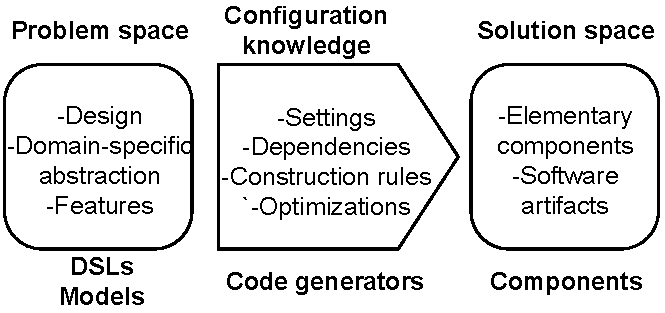
\includegraphics[scale=0.65]{Background/fig/GDM.pdf}
	\caption{Overview of the Docker-based testing architecture}
\end{figure}

\textbf{Among the main contributions of this thesis is to verify the correct mapping between the problem space and solution space. In other words, we would evaluate the impact of applied configurations during code transformation (by wether code generators or compilers) on the resource usage requirements.
}

In the following section, we present a general overview of the complete software development tool chain and the main actors that are involved from design time to runtime.


\section{An overview of the software development tool chain}
%\subsection{Automatic code generation}
\begin{figure}[h]
	\center
	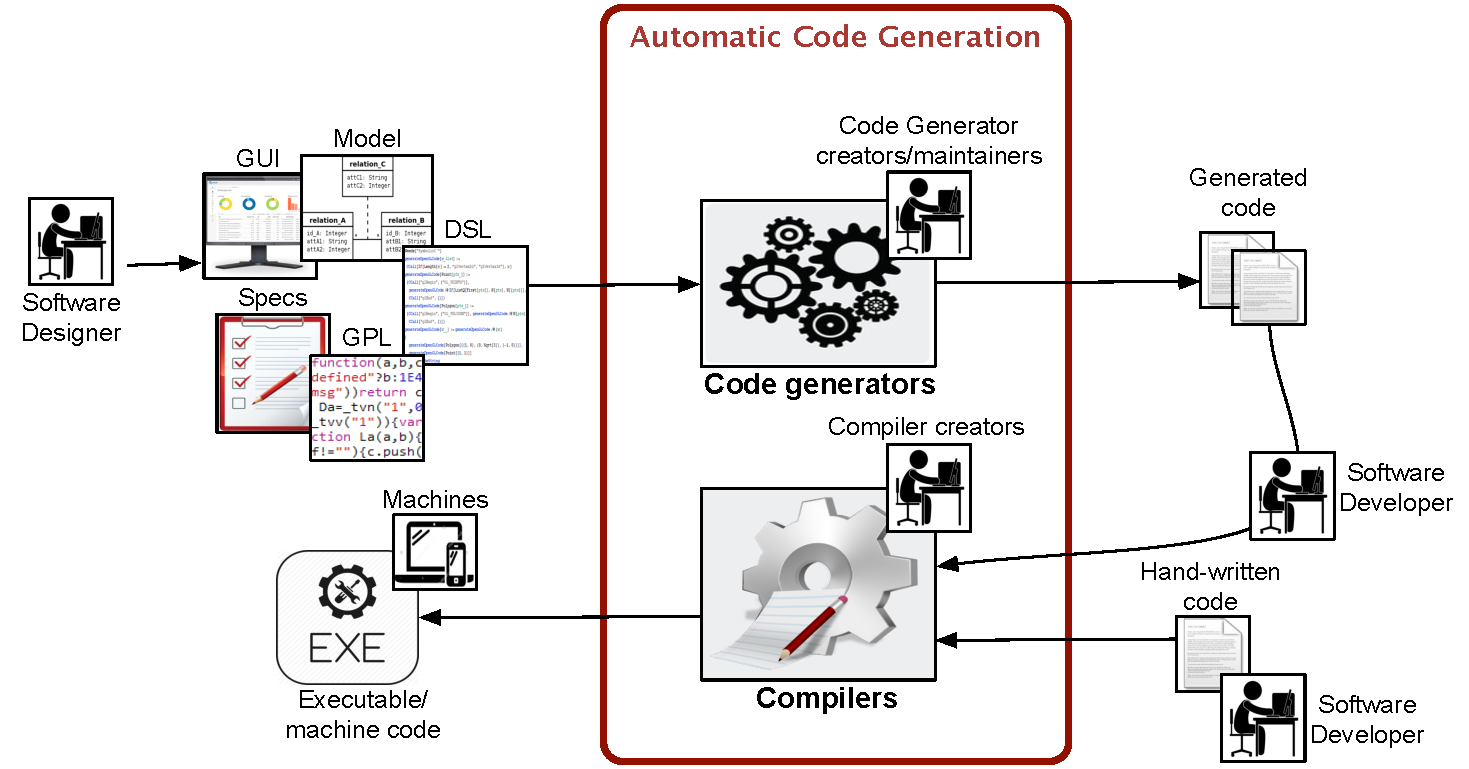
\includegraphics[scale=0.65]{Background/fig/background_overview2.pdf}
	\caption{Overview of the Docker-based testing architecture}
\end{figure}
The process of generative software development involves many different technologies. In this section, we describe in more details the different activities and actors involved to transform high-level specification into executable programs and that from design time to runtime. 
Figure 2.2 reviews the different steps of this chain. We distinguish four main tasks: 
\begin{itemize}
\item \textit{Software design:} 

As part of the generative programming process, the first step consists on representing the system behavior. 
Software design/behavior is the input program for the code generators. On the input side we can either use code as the input or an abstract form that represents the design. It depends on the type of the code generator and on the input source program it requires. These programs can range from a formal specification of the system behavior to abstract models that represents the business logic.
For example, software designers define, at design time, software’s behavior using for example Domain-Specific Models (DSMs), DSLs, Models, etc.
A DSM, as an example, is a system of abstractions that describes selected aspects of a sphere of knowledge and real-world concepts pertinent to the domain that need to be modeled in software. These models are specified using a high-level abstract languages (DSLs). %Domain-specific languages (DSLs) improve programmer productivity by providing high-level abstractions for the development of applications in a particular domain. Furthermore, software design can be provided as GUIs, GPLs, Models, etc.

\item \textit{Code generation:} 
Code generation is the technique of building code using programs. The common feature of the generator is to produce code that the software developer would otherwise write by hand.
There is no one style of code generation. Generators are generally seen as a black box which requires as input a program and generate as output a source code for a specific target software platform/language. Generators can work on the command line or using a GUI. 
Code generation can build code for one or more target language, once or multiple times. There are different varieties of code generation aspects and it highly depends on the type of the input programs described in the previous step. 
%Code generation techniques depends generally on these inputs.  
For example, code generator developers use model-driven techniques in order to generate automatically code. Thus, instead of focusing their efforts on constructing code, they build models and, in particular, create model transformations that transform these models into new models or code. Thus, the code generation process start by taking the previously defined specification to translate a model to an implementation in a target language. We will see in the next section the different types of code generators.


%In general, there are two main categories of Automatic code generation: passive or active.  Passive code generators build the code once, then have nothing more to do with the code.  It is up to the discretion of the user as to how to update and maintain the code.  Active code generators, on the other hand, keep track of the code during its lifecycle.  Active code generators are run on code multiple times during the lifecycle.  With Active Code generators, there is code you can modify, and code that should only be modified by the code generator.  Code generators can be further classified into code mungers, inline code expanders, mixed code generators, partial class generators, tier generators and domain languages\cite{fertalj2008source}. 

\item \textit{Software development:}
Software development may be divided into two main parts. On the one hand, software developers may follow the two previous steps in order to generate automatically code for a specific target software platform. In this case, they use to edit the system behavior in the first step (at a high level) and use to re-generate code each time needed by calling a specific generator. Generated code can even be edited in some cases by the end software developers. This task really depends on the complexity of the generated code and it sometimes need software experts that can easily update and maintain the code. On the other hand, they may manually implement source code from scratch without using any abstractions or code generation aspects. In this case, they just need to compile and execute the hand-written code in order to test it.
\item \textit{Compilation:}
Once code is generated or implemented, a classical compiler is used to translate the generated code into an executable. This translation depends on the target hardware platforms and it is up to the software developer to select the adequate compiler to use. Compilers are needed to target heterogeneous and diverse kinds of hardware architectures and devices. As an example, cross compilers may be used to create executable code for a platform other than the one on which the compiler is running. In case the generated code need to run on different machines/devices, the software developer need to use different compilers for each target software platform and deploy the generated executables within different machines which is a tedious and complicated task.
\end{itemize} 
.
%\begin{figure}[h]
%\center
%	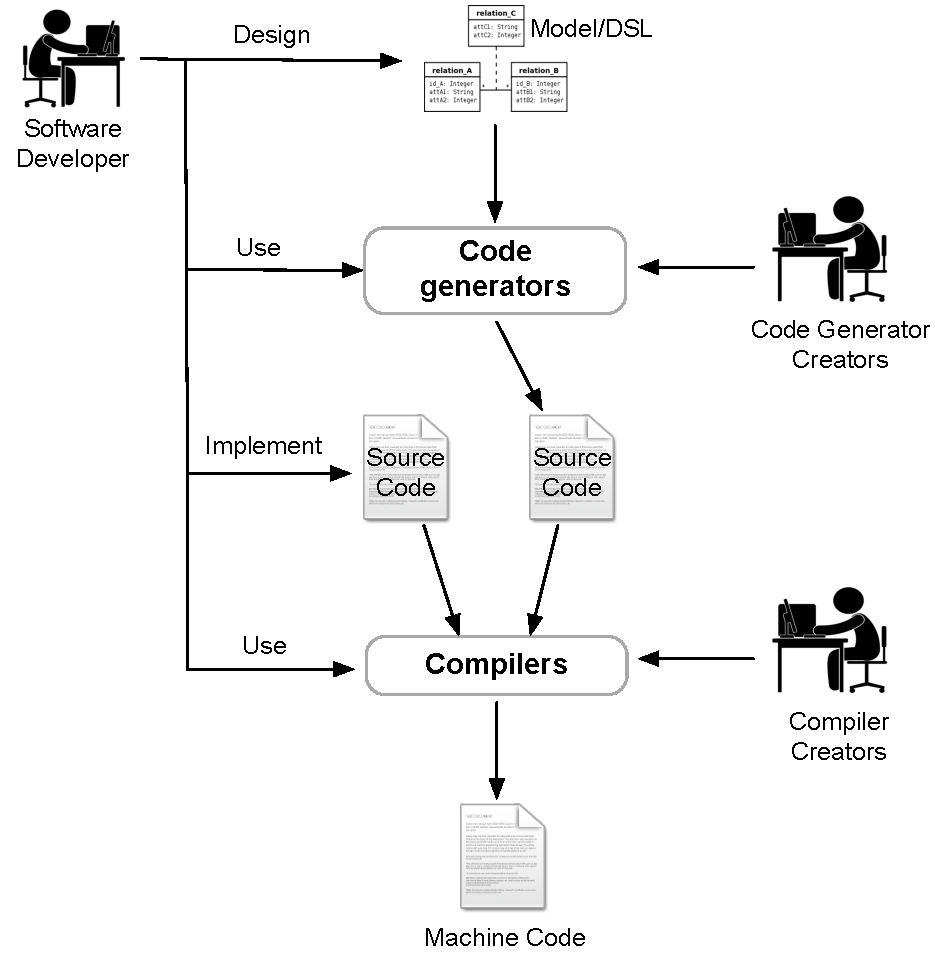
\includegraphics[scale=0.65]{Background/fig/background_overview.pdf}
%	\caption{Overview of the Docker-based testing architecture}
%\end{figure}
\section{Testing code generators}
\subsection{Code generation workflow}
In this thesis, we focus on testing the automatic code generation (highlighted with red box in figure 2.2). As stated before, the code generation workflow is divided into two levels. It starts by transforming the system design to source code through the use of generators. Afterwards, source code is transformed into executables using compilers. Thus, software developers use to generate code, edit it (if needed), compile it and then test it. If changes are applied to compilers or generators, the cycle is repeated. In the following sections, we give an overview of the types and properties of compilers and generators we would to test. Figure 2.3 presents an overview of this testing cycle. The right-hand side of the figure shows the classic workflow for developing and debugging code which is \textit{“edit, compile, and test.”}. The user writes or edits an existing code, compile it using specific compilers, and test it. Code generation adds a few new workflow elements in the left-hand side of the figure where generator creators edit the templates and definition files (or the generator itself) and then run the generator to create new output files. The output files are then compiled and the application is tested. 
\begin{figure}[h]
	\center
	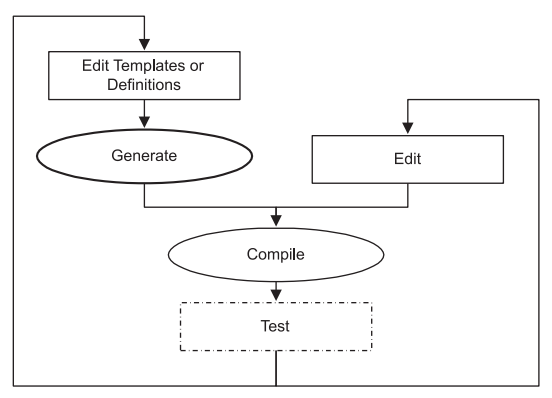
\includegraphics[scale=1]{Background/fig/workflow}
	\caption{Code generation workflow}
\end{figure}

The main goal of generators is to produce software systems from higher-level specifications. Generators bridge the wide gap between the high-level system description and the executable.
\subsection{Types of code generators}
There are many ways to categorize generators. We can differentiate them by their complexity, by usage, or by their input/output. According to\cite{herrington2003code} there are two main categories of automatic code generation: passive or active. Passive code generators build the code only once, then it’s up to the user to update and maintain the code.  Active code generators, run on code multiple times during the lifecycle.  With Active Code generators, there is code you can modify, and code that should only be modified by the code generator. With the active generator you first run the generator, then compile and test the output. At this point if you find a problem in the generated code, you alter the templates or input of the generator and re-generate. Active code generators are widely used in the literature. We focus on this thesis on testing active code generators.
There are six categories of active code generators: 

\begin{itemize}
\item Code munger: A code munger reads code as input and then builds new code as output. This new code can either be partial or complete depending on the design of the generator.
A code munger is the most common form of code generators and are used widely. This kind of generators are often used for automatically generating documentations.
A source-to-source compiler, transcompiler or transpiler \footnote{\url{"https://en.wikipedia.org/wiki/Source-to-source_compiler"}} can also be defined as code mungers. A transcompiler takes a code written in some programming language and translates it to a code written in some other language.

Examples:  C2J, JavaDoc, Jazillian, Closure Compiler, Coccinelle, CoffeeScript, Dart, Haxe, TypeScript and Emscripten



\item Inline code expander: This model reads code as input and the builds new code that uses the input code as a base but has sections of the code expanded based on designs in the original code. Embedded SQL languages, like Pro*C, are examples on inline code expanders. The SQL is written in the C code and the generator builds production C code by expanding the SQL into C code which implements the commands and queries.
Embedded SQL is a method of combining the computing power of a high-level language like Java or C/C++ and the database manipulation capabilities of SQL. 
It allows you to execute any SQL statement from an application program. 
In the example code, SQL is embedded into C source code files using special markup. These hybrid C files are given their own extension, such as '.sqlc‘:
 

\item Mixed code generator: This model use code as input and then builds new code using the input code as a base, but returning the output code back into the input file. Wizards are often implemented as mixed code generators. Special comments are embedded in the code which define regions where the generator adds new code. 

\item Partial class generator: A partial class generator takes an abstract definition as input and then builds output code which is meant to be extended by the user by sub-classing the output code and extending methods to complete the design. 

\item Tier generator: In this model the generator builds a complete set of output code from an abstract definition. This code is meant to be used as-is without extension. This is the most common form of open source and productized generator.

\item Full-domain language: Domain languages are basically new languages that are used for a specific type of problem.  Domain languages are the extreme end of automatic code generation because you basically have to write a compiler for your problem. 

\end{itemize}
%Generators are based on domain-specific models which define the semantics of the system specification language and also contain the knowledge of how to produce efficient implementations[REF]. 
%We distinguish two major types of code generators: rule-based model-to-model transformation languages (such as ATL) and template-based model-to-text transformation languages (such as Acceleo) to translate high-level system specifications into executable code and scripts.
\subsection{Complexity}
The complexity of code generators remains on the transformation rules and code generation process. In fact, code generators can be difficult to understand since they are typically composed of numerous elements, whose complex interdependencies pose important challenges for developers performing design, implementation, and maintenance tasks. 
Given the complexity and heterogeneity of the technologies involved in a code generator, developers who are trying to inspect and understand the code-generation process have to deal with numerous different artifacts. As an example, in a code-generator maintenance scenario, a developer might need to find all chained model-to-model and model-to-text transformation bindings, that originate a buggy line of code to fix it. This task is error prone when done manually. We believe that flexible traceability tools are needed to collect and visualize information about the architecture and operational mechanics of code generators, to reduce the challenges that developers face during their life-cycle.[ref W]

Moreover, the generated code has to meet certain performance requirements (e.g. execution speed, response time, memory consumption, utilization of resources, etc.). The challenge is that the structure of the specification is usually very different from the structure of the implementation: there is no simple one-to-one correspondence between the concepts in the specification and the concepts in the implementation. 
Efficient implementations are then computed at generation time by applying domain-specific optimizations and replacing, merging, adding, and removing components.

\begin{figure}[h]
	\center
	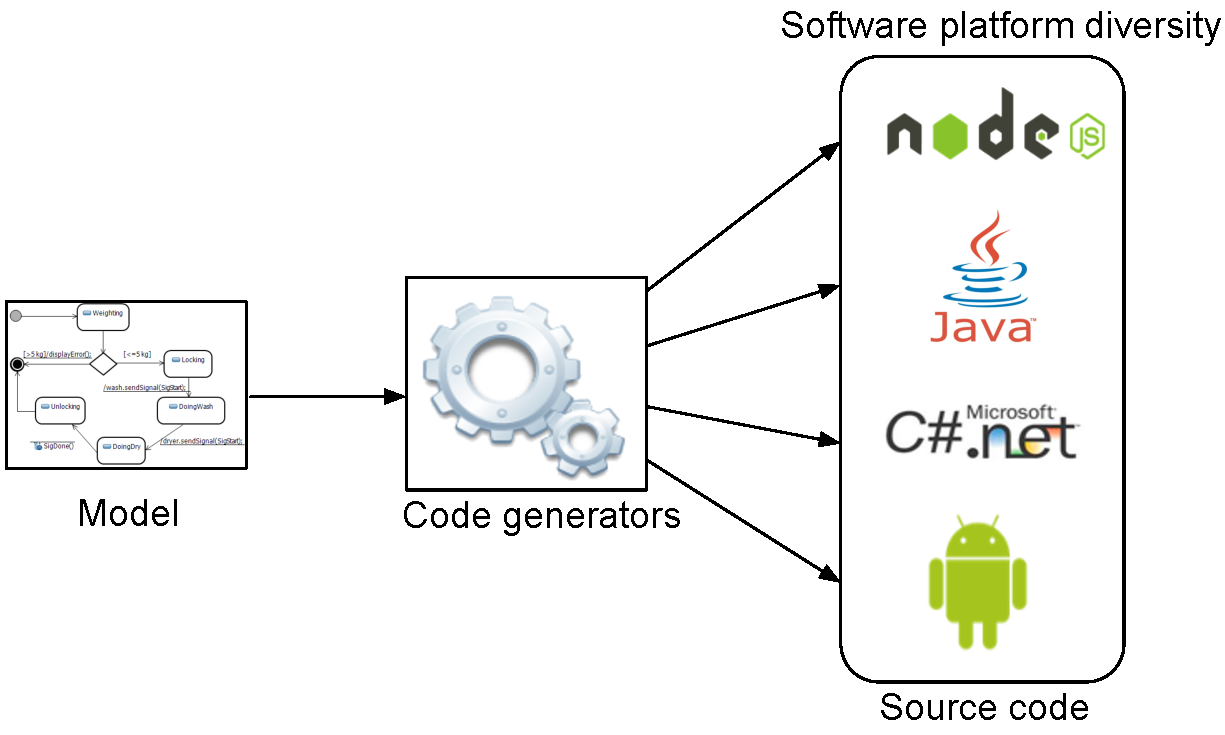
\includegraphics[scale=0.65]{Background/fig/software-diversity.pdf}
	\caption{Overview of the Docker-based testing architecture}
\end{figure}


\textbf{Challenge}: Fully automatic program synthesis offers many gains over traditional software development methods. e.g., speed of development, increased adaptability and reliability. But code generators are complex pieces of software themselves that may contain bugs.
\begin{itemize}
\item Can you trust the code-generator?
\item How can the correctness of the generated code be verified?
\end{itemize}

\section{Compilers auto-tuning}
The compilation is a process that translates a program in one language (the source
language) into an equivalent program in another language (target language). 
%Same as code generators, 
Commonly, the source language is a high-level programming language (i.e. a problem-oriented language), and the target language is a machine language or assembly language.
The key feature of compilers is to bridge source programs written in high-level languages with the underlying hardware architecture.
%\subsection{Types of code generators}
\begin{figure}[h]
	\center
	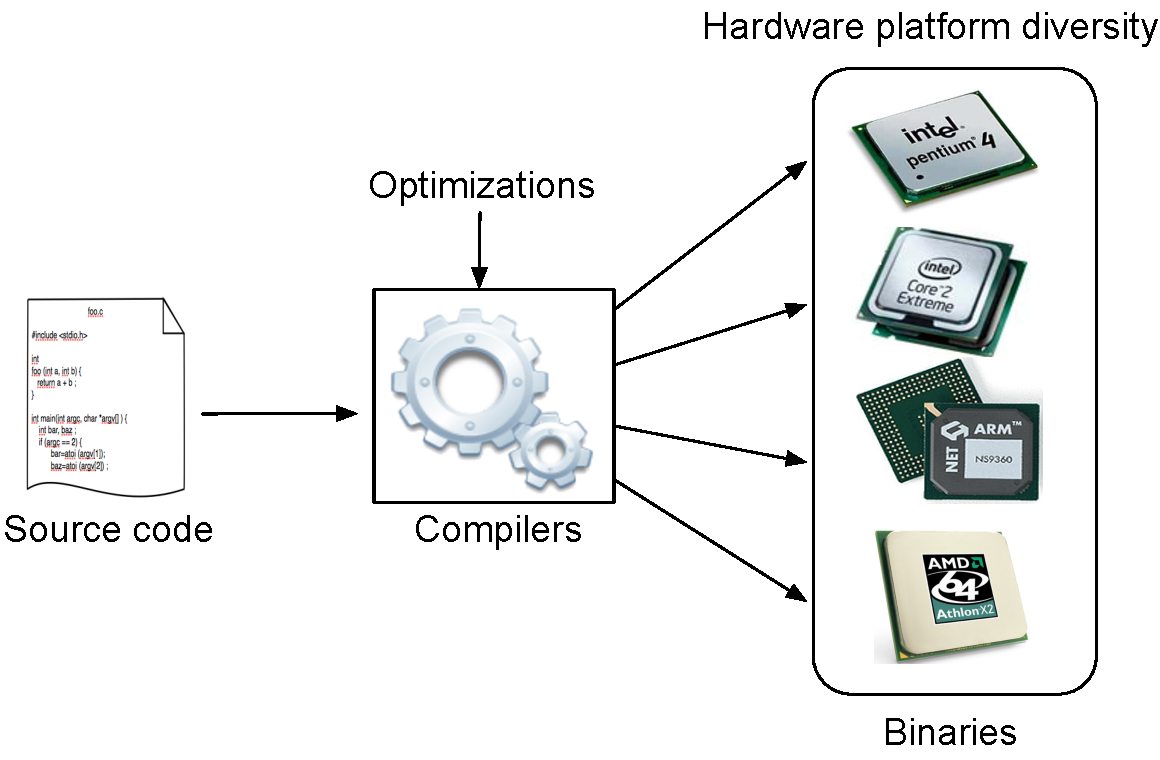
\includegraphics[scale=0.65]{Background/fig/hardware-diversity.pdf}
	\caption{Overview of the Docker-based testing architecture}
\end{figure}


\subsection{Complexity}
Modern compilers implement a number of optimizations. Each optimization tries to improve the performance of certain target applications. Improvement of source code programs in terms of performance can refer to several different non-functional properties of the produced code such as code size, resource or energy consumption, execution time, among others~\cite{almagor2004finding,pan2006fast}.
Testing non-functional properties is more challenging 
Thus, the determination of optimal settings of compiler optimizations has been identified as a major problem because compilers may have a huge number of potential optimization combinations, making it hard and time-consuming for software developers to find/construct the sequence of optimizations that satisfies user specific key objectives and criteria. It also requires a comprehensive understanding of the underlying system architecture, the target application, and the available optimizations of the compiler.







%\section{Compilers and Code generators non-functional testing}
\section{Testing challenges}

\begin{itemize}
	\item Auto-tuning compilers: Choosing which optimization the user should apply? Evaluate the efficiency of generated code? All these questions make the activity of testing compilers very challenging.
	\item Detecting bugs in code generators: How to automatically detect issues wthin code generators? Proving that the generated code is functionally correct is not enough to claim the effectiveness of the code generator under test?
	\item Resource usage monitoring of generated code: Due to the software and hardware heterogeneity, monitoring the resource usage of each execution platform is still challenging and time-consuming. 
%\subsection{Resource usage monitoring}
\end{itemize}


%metamorphic testing
%CG vs compilers 
%reorganisation
%comment olivier
%famille de GC
